\chapter*{Vita}
{\bfseries\large Jean-Pierre Serre}\\
Professor of Algebra and Geometry at the Collège de France, Paris, was born in
Bagcs, France, on September 15, 1926. He graduated from École Normale
Superieure, Paris, in 1948, and obtained his Ph.D. from the Sorbonne in 1951.
In 1954 he was awarded a Fields Medal for his work on topology (homotopy
groups) and algebraic geometry (coherent sheaves). Since then, his main topics
of interest have been number theory, group theory, and modular forms. Professor
Serre has been a frequent visitor of the United States, especially at the
Institute for Advanced Study, Princeton, and Harvard University. He is a
foreign member of the National Academy of Sciences of the U.S.A.

\chapter*{Preface to the second edition}
The present edition differs from the original one (published in 1968) by:
\begin{itemize}
	\item the inclusion of short notes giving references to new results;
	\item a supplementary bibliography.
\end{itemize}
Otherwise, the text has been left unchanged, except for the correction of a few
misprints.

The added bibliography does not claim to be complete. Its aim is just to help
the reader get acquainted with some of the many developments of the past twenty
years (for those prior to 1977, see also the survey \cite{78}). Among these
developments, one may especially mention the following:

\section*{\texorpdfstring{$\ell$}{ℓ}-adic representations associated to abelian
varieties over number fields}
Deligne (cf.\ \cite{52}) has proved that Hodge cohomology classes behave under
the action of the Galois group as if they were algebraic, thus providing a very
useful substitute for the still unproved Hodge conjecture.

Faltings (\cite{54}, see also \citeauthor{82}~\cite{82} and
\citeauthor{56}~\cite{56}), has proved Tate's conjecture that the map
\[
	\Hom_K(A, B) \otimes_\Z \Z_\ell \longrightarrow
	\Hom_{\Gal(\algcl\Q/K)}(T_\ell(A), T_\ell(B))
\]
is an isomorphism ($A$ and $B$ being abelian varieties over a number field
$K$), together with the semi-simplicity of the Galois module $Q_\ell
\otimes_{\Z_\ell} T_\ell(A)$ and similar results for $T_\ell(A)/\ell T_\ell(A)$
when $\ell$ is large enough. These results may be used to study the structure
of the Galois group of the division points of $A$, cf.\ \cite{80}. For
instance, if $\dim A$ is odd and $\End_KA = \Z$, one can show that this Galois
group has finite index in the group of symplectic similitudes; for elliptic
curves, i.e.\ $\dim A = 1$, this was already proved in \cite{76}.

\section*{Modular forms and \texorpdfstring{$\ell$}{ℓ}-adic representations}
The existence of $\ell$-adic representations attached to modular forms,
conjectured in the first edition of this book, has been proved by Deligne
(\cite{50}, see also Langlands~\cite{65} and Carayol~\cite{49}). This has many
applications for instance to the Ramanujan conjecture (Deligne) and to
congruence properties (Ribet \cite{69}, \cite{71}; Swinnerton-Dyer \cite{81};
\cite{73}, \cite{77}). Some generalizations are known (e.g.\ Carayol \cite{49};
Ohta \cite{68}; Wiles \cite{84}), but one can hope for much more, in the
setting of \textquote{Langlands' program}: there should exist a
% \missingfigure{Diagram of Langlands' program.}
\begin{figure}[!hbt]
	\centering
	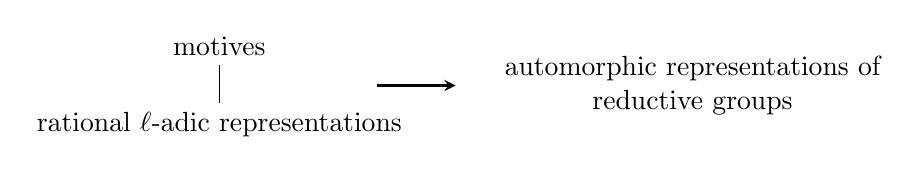
\begin{tikzpicture}
		\node (mot) at (0, 0) {motives};
		\node (l_adic) at (0, -1) {rational $\ell$-adic representations};
		\node[anchor=west, align=center] (auto) at (3.5, -.5) {automorphic representations of\\reductive groups};
		% \draw (mot) --node[sloped, above]{$\sim$} (l_adic);
		\draw (mot) -- (l_adic);
		\draw[thick, -stealth] (2.5, -.5) +(-.5, 0) -- +(.5, 0);
	\end{tikzpicture}
\end{figure}

\noindent
where the vertical line is (essentially) bijective and the horizontal arrow
injective with a precise description of its image (Deligne \cite{51}; Langlands
\cite{66}; \cite{78}). Such a diagram would incorporate, among other things,
the conjectures of Artin (on the holomorphy of $L$-functions) and Taniyama-Weil
(on elliptic curves over $\Q$). Chapters~\ref{ch:ii} and \ref{ch:iii} of the
presentbook, supplemented by the results of Deligne (\cite{53}) and Waldschmidt
(\cite{63}, \cite{83}), may be viewed as a partial realization of this
ambitious program in the abelian case.

\section*{Local theory of \texorpdfstring{$\ell$}{ℓ}-adic representations}
Here the ground field $K$, instead of being a number field, is a local field of
residue characteristic $p$. The most interesting case is $\char K = 0$ and $p =
\ell$, especially when a Hodge-Tate decomposition exists: indeed this gives
precious information on the image of the inertia group (Sen \cite{72};
\cite{79}; Wintenberger \cite{85}). When the $\ell$-adic representation comes
from a divisible group or an abelian variety, the existence of such a
decomposition is well known (Tate \cite{39}; see also Fontaine \cite{60}); for
representations coming from higher dimension cohomology, it has been proved
recently by Fontaine-Messing (under some restrictions, cf.\ \cite{62}) and
Faltings (\cite{55}). The results of Fontaine-Messing are parts of a
vastprogram by Fontaine, relating Galois representations and modules of
Dieudonné type (over some \textquote{Barsotti-Tate rings}, cf.\ \cite{58},
\cite{59}, \cite{61}).
